\begin{enumerate}[label=\thesection.\arabic*,ref=\thesection.\theenumi]
\numberwithin{equation}{enumi}
\numberwithin{figure}{enumi}
\numberwithin{table}{enumi}
\item Find the angle between two vectors $\overrightarrow{a}$ and $\overrightarrow {b} $ with magnitudes $\sqrt{3}$ and 2 respectively having $\overrightarrow {a}.\overrightarrow {b}=\sqrt{6}$.
	\\
	\solution
		\iffalse
\documentclass[10pt]{article}
\usepackage{graphicx}
\usepackage[none]{hyphenat}
\usepackage{graphicx}
\usepackage{listings}
\usepackage[english]{babel}
\usepackage{siunitx}
\usepackage{graphicx}
\usepackage{caption} 
\usepackage{booktabs}
\usepackage{array}
\usepackage{amssymb} % for \because
\usepackage{amsmath}   % for having text in math mode
\usepackage{extarrows} % for Row operations arrows
\usepackage{listings}
\usepackage[utf8]{inputenc}
\lstset{
  frame=single,
  breaklines=true
}
\usepackage{hyperref}
  
%Following 2 lines were added to remove the blank page at the beginning
\usepackage{atbegshi}% http://ctan.org/pkg/atbegshi
\AtBeginDocument{\AtBeginShipoutNext{\AtBeginShipoutDiscard}}


%New macro definitions
\newcommand{\mydet}[1]{\ensuremath{\begin{vmatrix}#1\end{vmatrix}}}
\providecommand{\brak}[1]{\ensuremath{\left(#1\right)}}
\newcommand{\solution}{\noindent \textbf{Solution: }}
\newcommand{\myvec}[1]{\ensuremath{\begin{pmatrix}#1\end{pmatrix}}}
\providecommand{\norm}[1]{\left\lVert#1\right\rVert}
\providecommand{\abs}[1]{\left\vert#1\right\vert}
\let\vec\mathbf{}
\begin{document}

\begin{center}
\title{\textbf{VECTORS}}
\date{\vspace{-5ex}} %Not to print date automatically
\maketitle
\end{center}

\section{12$^{th}$ Maths - EXERCISE-10.3}

\begin{enumerate}
\item Find the angle between two vectors $\overrightarrow{a}$ and $\overrightarrow {b} $ with magnitudes $\sqrt{3}$ and 2 respectively having $\overrightarrow {a}.\overrightarrow {b}=\sqrt{6}$.\\  

\solution
\fi
From the given information,
\begin{align}
\norm{\vec{a}}&=\sqrt{3}\\
\norm{\vec{b}}&= 2\\
{\vec{a}^{\top}}{\vec{b}}&=\sqrt{6}  
\end{align}
Thus,
\begin{align}
\cos\theta&=\frac{{\vec{a}^{\top}}{\vec{b}}}{\norm{\vec{a}}\norm{\vec{b}}}\\
&=\frac{1}{\sqrt{2}}\\
\implies\theta&={45}\degree
\end{align}

\item Find the angle between the the vectors $\hat{i}-2\hat{j}+3\hat{k}$ and $3\hat{i}-2\hat{j}+\hat{k}$.
	\\
	\solution
		\iffalse
\documentclass[journal,12pt]{article}
\usepackage{graphicx}
\usepackage[none]{hyphenat}
\usepackage{graphicx}
\usepackage{listings}
\usepackage[english]{babel}
\usepackage{siunitx}
\usepackage{graphicx}
\usepackage{caption} 
\usepackage{booktabs}
\usepackage{array}
\usepackage{amssymb} % for \because
\usepackage{amsmath}   % for having text in math mode
\usepackage{extarrows} % for Row operations arrows
\usepackage{listings}
\usepackage[utf8]{inputenc}
\lstset{
  frame=single,
  breaklines=true
}
\usepackage{hyperref}
  
%Following 2 lines were added to remove the blank page at the beginning
\usepackage{atbegshi}% http://ctan.org/pkg/atbegshi
\AtBeginDocument{\AtBeginShipoutNext{\AtBeginShipoutDiscard}}


%New macro definitions
\newcommand{\mydet}[1]{\ensuremath{\begin{vmatrix}#1\end{vmatrix}}}
\providecommand{\brak}[1]{\ensuremath{\left(#1\right)}}
\newcommand{\solution}{\noindent \textbf{Solution: }}
\newcommand{\myvec}[1]{\ensuremath{\begin{pmatrix}#1\end{pmatrix}}}
\providecommand{\norm}[1]{\left\lVert#1\right\rVert}
\providecommand{\abs}[1]{\left\vert#1\right\vert}
\let\vec\mathbf

\begin{document}

\begin{center}
\title{\textbf{VECTORS}}
\date{\vspace{-5ex}} %Not to print date automatically
\maketitle
\end{center}

\section*{$12^{th}$ Maths - EXERCISE-10.3}

\begin{enumerate}
\item Find the angle between the vectors $\\ \overrightarrow{a}=\hat{i}-2\hat{j}+3\hat{k}$ and $\overrightarrow{b}=3\hat{i}-2\hat{j}+\hat{k}$  
\section*{solution}
\fi
Let the given points be
\begin{align}
	\vec{a} &= \myvec{1\\-2\\3} , \vec{b} = \myvec{3\\ -2 \\ 1},
\end{align}
Since 
\begin{align}
\vec{a}^{\top}\vec{b}=10, \,
\norm{\vec{a}}=\sqrt{14}, \, 
	\norm{\vec{b}}&=\sqrt{14}, 
\label{eq:chapters/12/10/3/2/5}
\\
\cos\theta=\frac{\vec{a}^{\top}\vec{b}}{\norm{\vec{a}}\norm{\vec{b}}}
	&= \frac{5}{7}
	\\
	\implies \theta&= \cos^{-1}\frac{5}{7}
\end{align}

\item Find $\abs{\overrightarrow {a}}$ and $\abs{\overrightarrow {b}}$,if ($\overrightarrow {a}+\overrightarrow {b}).(\overrightarrow {a}-\overrightarrow {b})=8$ and $\abs{\overrightarrow {a}}=8\abs{\overrightarrow {b}}$.
	\\
	\solution
		\iffalse
\documentclass[10pt]{article}
\usepackage{graphicx}
\usepackage[none]{hyphenat}
\usepackage{graphicx}
\usepackage{listings}
\usepackage[english]{babel}
\usepackage{siunitx}
\usepackage{graphicx}
\usepackage{caption} 
\usepackage{booktabs}
\usepackage{array}
\usepackage{amssymb} % for \because
\usepackage{amsmath}   % for having text in math mode
\usepackage{extarrows} % for Row operations arrows
\usepackage{listings}
\usepackage[utf8]{inputenc}
\lstset{
  frame=single,
  breaklines=true
}
\usepackage{hyperref}
  
%Following 2 lines were added to remove the blank page at the beginning
\usepackage{atbegshi}% http://ctan.org/pkg/atbegshi
\AtBeginDocument{\AtBeginShipoutNext{\AtBeginShipoutDiscard}}


%New macro definitions
\newcommand{\mydet}[1]{\ensuremath{\begin{vmatrix}#1\end{vmatrix}}}
\providecommand{\brak}[1]{\ensuremath{\left(#1\right)}}
\newcommand{\solution}{\noindent \textbf{Solution: }}
\newcommand{\myvec}[1]{\ensuremath{\begin{pmatrix}#1\end{pmatrix}}}
\providecommand{\norm}[1]{\left\lVert#1\right\rVert}
\providecommand{\abs}[1]{\left\vert#1\right\vert}
\let\vec\mathbf{}
\begin{document}

\begin{center}
\title{\textbf{VECTORS}}
\date{\vspace{-5ex}} %Not to print date automatically
\maketitle
\end{center}

\section{12$^{th}$ Maths - EXERCISE-10.3}

\begin{enumerate}
\item Find $\abs{\overrightarrow{a}}$ and $\abs{\overrightarrow{b}}$, if ($\overrightarrow{a}$+$\overrightarrow{b}$)$.$($\overrightarrow{a}$-$\overrightarrow{b}$)=8 and $\abs{\overrightarrow{a}}$=8$\abs{\overrightarrow{b}}$.\\  

\solution
\fi
Since
\begin{align}
\brak{\vec{a}+\vec{b}}^\top\brak{\vec{a}-\vec{b}}&=8,\\
\norm{\vec{a}}^2-\norm{\vec{b}}^2&=8\\
\implies\norm{8\vec{b}}^2-\norm{\vec{b}}^2&=8\\
\implies \norm{\vec{b}}&=\frac{2\sqrt{2}}{3\sqrt{7}}
\end{align}
Thus, 
\begin{align}
\norm{\vec{a}}&=8\norm{\vec{b}}
=\frac{16\sqrt{2}}{3\sqrt{7}}
\end{align}

\item Evaluate the product(3$\overrightarrow {a}-5\overrightarrow {b}).(2\overrightarrow {a}+7\overrightarrow {b}$).
	\\
	\solution
		\iffalse
\documentclass[12pt]{article}\usepackage{graphicx}
\graphicspath{{./figs/}}{}

\usepackage{amsmath,amssymb,amsfonts,amsthm}
\newcommand{\myvec}[1]{\ensuremath{\begin{pmatrix}#1\end{pmatrix}}}
%\providecommand{\norm}[1]{\lVert#1\rVert}3
\usepackage{listings}
\usepackage{watermark}
\usepackage{titlesec}
\usepackage{caption}
\let\vec\mathbf
\lstset{
frame=single, 
breaklines=true,
columns=fullflexible
}
\usepackage{atbegshi}% http://ctan.org/pkg/atbegshi
\AtBeginDocument{\AtBeginShipoutNext{\AtBeginShipoutDiscard}}
\let\vec\mathbf
\providecommand{\norm}[1]{\left\lVert#1\right\rVert}
\providecommand{\qfunc}[1]{\ensuremath{Q\left(#1\right)}}
\providecommand{\sbrak}[1]{\ensuremath{{}\left[#1\right]}}
\providecommand{\lsbrak}[1]{\ensuremath{{}\left[#1\right.}}
\providecommand{\rsbrak}[1]{\ensuremath{{}\left.#1\right]}}
\providecommand{\brak}[1]{\ensuremath{\left(#1\right)}}
\providecommand{\lbrak}[1]{\ensuremath{\left(#1\right.}}
\providecommand{\rbrak}[1]{\ensuremath{\left.#1\right)}}
\providecommand{\cbrak}[1]{\ensuremath{\left\{#1\right\}}}
\providecommand{\lcbrak}[1]{\ensuremath{\left\{#1\right.}}
\providecommand{\rcbrak}[1]{\ensuremath{\left.#1\right\}}}
\newcommand{\solution}{\noindent \textbf{Solution: }}
\newcommand{\mydet}[1]{\ensuremath{\begin{vmatrix}#1\end{vmatrix}}}
\title{\mytitle}
\begin{document}
\begin{center}
\title{\textbf{VECTOR ALGEBRA}}
\maketitle
\end{center}
\begin{enumerate}
\item\textbf{Problem statement :} Evaluate the product $\brak{3\overrightarrow{a}-5\overrightarrow{b}}\cdot\brak{2\overrightarrow{a}+7\overrightarrow{b}}$
\solution
\fi
\begin{multline}
    \brak{3\vec{a}-5\vec{b}}^{\top}\brak{2\vec{a}+7\vec{b}}= \brak{3\vec{a}^{\top}}\brak{2\vec{a}}+\brak{3\vec{a}^{\top}}\brak{7\vec{b}}-\brak{5\vec{b}^{\top}}\brak{2\vec{a}}-\brak{5\vec{b}^{\top}}\brak{7\vec{b}}
    \\
     = 6\norm{\vec{a}}^2 +21\vec{a}^{\top}\vec{b}-10\vec{b}^{\top}\vec{a}-35\norm{\vec{b}}^2 
     =6\norm{\vec{a}}^2-35\norm{\vec{b}}^2+11\vec{a}^{\top}\vec{b}
\end{multline}

\item Find the magnitude of two vectors $\overrightarrow {a}$ and $\overrightarrow {b}$, having the same magnitude and such that the angle between them is $60\degree$ and their scalar product is $\frac{1}{2}$
	\\
	\solution
		\iffalse
\documentclass[10pt]{article}
\usepackage{graphicx}
\usepackage[none]{hyphenat}
\usepackage{listings}
\usepackage[english]{babel}
\usepackage{siunitx}
\usepackage{caption}
\usepackage{booktabs}
\usepackage{array}
\usepackage{extarrows}
\usepackage{enumerate}
\usepackage{enumitem}
\usepackage{amsmath}
\usepackage{commath}
\usepackage{gensymb}
\usepackage{amssymb}
\usepackage{multicol}
\usepackage[utf8]{inputenc}
\lstset{
	frame=single,
	breaklines=true
}
\usepackage{hyperref}
%\usepackage[margin=0.8in]{geometry}
%\usepackage{exsheets}% also loads the `tasks' package
\usepackage{atbegshi}
\AtBeginDocument{\AtBeginShipoutNext{\AtBeginShipoutDiscard}}

%new macro definitions
\newcommand{\mydet}[1]{\ensuremath{\begin{vmatrix}#1\end{vmatrix}}}
\providecommand{\brak}[1]{\ensuremath{\left(#1\right)}}
\newcommand{\solution}{\noindent \textbf{Solution: }}
\newcommand{\myvet}[1]{\ensuremath{\begin{pmatrix}#1\end{pmatrix}}}
\providecommand{\norm}[1]{\left\1Vert#1\right\rVert}
\let\vec\mathbf{}


%\SetEnumitemKey{twocol}{
%	before=\raggedcolumns\begin{multicols}{2},
%	after=\end{multicols}}
%\SetEnumitemKey{fourcol}{
%	before=\raggedcolumns\begin{multicols}{4},
%	after=\end{multicols}}	


\begin{document}
\begin{center}
\title{\textbf{VECTORS}}
\date{\vspace{-5ex}}
\maketitle
\end{center}
\section*{12$^{th}$Math - Chapter 10}
This is Problem-8 from Exercise 10.3\\\\
Find the magnitude of two vectors $\overrightarrow{a}$ and $\overrightarrow{b}$, having the same magnitude and such that the angle between them is 60 $\degree$ and their scalar product is $\dfrac{1}{2}$.

\solution
\fi
Given 
\begin{align}
\norm{\vec{a}}\norm{\vec{b}}&=\frac{{{\vec{a}}^{\top}}{\vec{b}}}{\cos\theta}\\
\implies 
\norm{\vec{a}}&=\sqrt{\frac{{\vec{a}}^{\top}{\vec{b}}}{\cos\theta}}\\
\end{align}
since 
\begin{align}
\norm{\vec{a}}=\norm{\vec{b}}
\end{align}
Substituting numerical values,
\begin{align}
\norm{\vec{a}}
= \norm{\vec{b}}=1
\end{align}

\item Find $\abs{\overrightarrow {x}}$,if for a unit vector $\overrightarrow {a},(\overrightarrow {x}-\overrightarrow {a}).(\overrightarrow {x}+\overrightarrow {a}$)=12.
	\\
		\iffalse
\documentclass[12pt]{article}
\usepackage{graphicx}
%\documentclass[journal,12pt,twocolumn]{IEEEtran}
\usepackage[none]{hyphenat}
\usepackage{graphicx}
\usepackage{listings}
\usepackage[english]{babel}
\usepackage{graphicx}
\usepackage{caption} 
\usepackage{hyperref}
\usepackage{booktabs}
\usepackage{array}
\usepackage{amsmath}   % for having text in math mode
\usepackage{listings}
\lstset{
  frame=single,
  breaklines=true
}
  
%Following 2 lines were added to remove the blank page at the beginning
\usepackage{atbegshi}% http://ctan.org/pkg/atbegshi
\AtBeginDocument{\AtBeginShipoutNext{\AtBeginShipoutDiscard}}
%


%New macro definitions
\newcommand{\mydet}[1]{\ensuremath{\begin{vmatrix}#1\end{vmatrix}}}
\providecommand{\brak}[1]{\ensuremath{\left(#1\right)}}
\providecommand{\norm}[1]{\left\lVert#1\right\rVert}
\newcommand{\solution}{\noindent \textbf{Solution: }}
\newcommand{\myvec}[1]{\ensuremath{\begin{pmatrix}#1\end{pmatrix}}}
\let\vec\mathbf

\begin{document}

\begin{center}
\title{\textbf{Vector Dot Product}}
\date{\vspace{-5ex}} %Not to print date automatically
\maketitle
\end{center}
\setcounter{page}{1}

\section{12$^{th}$ Maths - Chapter 10}
This is Problem-9 from Exercise 10.3
\begin{enumerate}
\item Find $\norm{\vec{x}}$, if for a unit vector $\vec{a}$, $\brak{\vec{x}-\vec{a}}.\brak{\vec{x}+\vec{a}} = 12$.\\
	\fi
\solution 
From the given information,
\begin{align}
  \label{eq:12/10/3/9det2f}
  \brak{\vec{x}-\vec{a}}^\top\brak{\vec{x}+\vec{a}} &= 12 \\
  \implies \vec{x}^\top\vec{x} - \vec{a}^\top\vec{x} + \vec{x}^\top\vec{a} - \vec{a}^\top\vec{a} &= 12 \\
  \implies \norm{\vec{x}}^{2} - \norm{\vec{a}}^{2} &= 12 \\
\implies   \norm{\vec{x}}^{2} - 1 &= 12  \\
	\text{or, }  
	\norm{\vec{x}} &= \sqrt{13}
\end{align}

\item If the vertices A,B,C of a triangle ABC are (1,2,3),(-1,0,0)(0,1,2), respectively , then find  $\angle{ABC}. [\angle{ABC}$ is the angle between the vectors $\overrightarrow{BA}$ and $\overrightarrow{BC}$].
	\\
	\solution
		\iffalse
\documentclass[journal,12pt,twocolumn]{IEEEtran}
%
\usepackage{setspace}
\usepackage{gensymb}
%\doublespacing
\singlespacing

%\usepackage{graphicx}
%\usepackage{amssymb}
%\usepackage{relsize}
\usepackage[cmex10]{amsmath}
%\usepackage{amsthm}
%\interdisplaylinepenalty=2500
%\savesymbol{iint}
%\usepackage{txfonts}
%\restoresymbol{TXF}{iint}
%\usepackage{wasysym}
\usepackage{amsthm}
%\usepackage{iithtlc}
\usepackage{mathrsfs}
\usepackage{txfonts}
\usepackage{stfloats}
\usepackage{bm}
\usepackage{cite}
\usepackage{cases}
\usepackage{subfig}
%\usepackage{xtab}
\usepackage{longtable}
\usepackage{multirow}
%\usepackage{algorithm}
%\usepackage{algpseudocode}
\usepackage{enumitem}
\usepackage{mathtools}
\usepackage{steinmetz}
\usepackage{tikz}
\usepackage{circuitikz}
\usepackage{verbatim}
\usepackage{tfrupee}
\usepackage[breaklinks=true]{hyperref}
%\usepackage{stmaryrd}
\usepackage{tkz-euclide} % loads  TikZ and tkz-base
%\usetkzobj{all}
\usetikzlibrary{calc,math}
\usepackage{listings}
    \usepackage{color}                                            %%
    \usepackage{array}                                            %%
    \usepackage{longtable}                                        %%
    \usepackage{calc}                                             %%
    \usepackage{multirow}                                         %%
    \usepackage{hhline}                                           %%
    \usepackage{ifthen}                                           %%
  %optionally (for landscape tables embedded in another document): %%
    \usepackage{lscape}     
\usepackage{multicol}
\usepackage{chngcntr}
%\usepackage{enumerate}

%\usepackage{wasysym}
%\newcounter{MYtempeqncnt}
\DeclareMathOperator*{\Res}{Res}
%\renewcommand{\baselinestretch}{2}
\renewcommand\thesection{\arabic{section}}
\renewcommand\thesubsection{\thesection.\arabic{subsection}}
\renewcommand\thesubsubsection{\thesubsection.\arabic{subsubsection}}

\renewcommand\thesectiondis{\arabic{section}}
\renewcommand\thesubsectiondis{\thesectiondis.\arabic{subsection}}
\renewcommand\thesubsubsectiondis{\thesubsectiondis.\arabic{subsubsection}}

% correct bad hyphenation here
\hyphenation{op-tical net-works semi-conduc-tor}
\def\inputGnumericTable{}                                 %%

\lstset{
%language=C,
frame=single, 
breaklines=true,
columns=fullflexible
}
%\lstset{
%language=tex,
%frame=single, 
%breaklines=true
%}

\begin{document}
%


\newtheorem{theorem}{Theorem}[section]
\newtheorem{problem}{Problem}
\newtheorem{proposition}{Proposition}[section]
\newtheorem{lemma}{Lemma}[section]
\newtheorem{corollary}[theorem]{Corollary}
\newtheorem{example}{Example}[section]
\newtheorem{definition}[problem]{Definition}
%\newtheorem{thm}{Theorem}[section] 
%\newtheorem{defn}[thm]{Definition}
%\newtheorem{algorithm}{Algorithm}[section]
%\newtheorem{cor}{Corollary}
\newcommand{\BEQA}{\begin{eqnarray}}
\newcommand{\EEQA}{\end{eqnarray}}
\newcommand{\define}{\stackrel{\triangle}{=}}

\bibliographystyle{IEEEtran}
%\bibliographystyle{ieeetr}


\providecommand{\mbf}{\mathbf}
\providecommand{\pr}[1]{\ensuremath{\Pr\left(#1\right)}}
\providecommand{\qfunc}[1]{\ensuremath{Q\left(#1\right)}}
\providecommand{\sbrak}[1]{\ensuremath{{}\left[#1\right]}}
\providecommand{\lsbrak}[1]{\ensuremath{{}\left[#1\right.}}
\providecommand{\rsbrak}[1]{\ensuremath{{}\left.#1\right]}}
\providecommand{\brak}[1]{\ensuremath{\left(#1\right)}}
\providecommand{\lbrak}[1]{\ensuremath{\left(#1\right.}}
\providecommand{\rbrak}[1]{\ensuremath{\left.#1\right)}}
\providecommand{\cbrak}[1]{\ensuremath{\left\{#1\right\}}}
\providecommand{\lcbrak}[1]{\ensuremath{\left\{#1\right.}}
\providecommand{\rcbrak}[1]{\ensuremath{\left.#1\right\}}}
\theoremstyle{remark}
\newtheorem{rem}{Remark}
\newcommand{\sgn}{\mathop{\mathrm{sgn}}}
\providecommand{\abs}[1]{\left\vert#1\right\vert}
\providecommand{\res}[1]{\Res\displaylimits_{#1}} 
\providecommand{\norm}[1]{\left\lVert#1\right\rVert}
%\providecommand{\norm}[1]{\lVert#1\rVert}
\providecommand{\mtx}[1]{\mathbf{#1}}
\providecommand{\mean}[1]{E\left[ #1 \right]}
\providecommand{\fourier}{\overset{\mathcal{F}}{ \rightleftharpoons}}
%\providecommand{\hilbert}{\overset{\mathcal{H}}{ \rightleftharpoons}}
\providecommand{\system}{\overset{\mathcal{H}}{ \longleftrightarrow}}
	%\newcommand{\solution}[2]{\textbf{Solution:}{#1}}
\newcommand{\solution}{\noindent \textbf{Solution: }}
\newcommand{\cosec}{\,\text{cosec}\,}
\providecommand{\dec}[2]{\ensuremath{\overset{#1}{\underset{#2}{\gtrless}}}}
\newcommand{\myvec}[1]{\ensuremath{\begin{pmatrix}#1\end{pmatrix}}}
\newcommand{\mydet}[1]{\ensuremath{\begin{vmatrix}#1\end{vmatrix}}}
%\numberwithin{equation}{section}
\numberwithin{equation}{subsection}
%\numberwithin{problem}{section}
%\numberwithin{definition}{section}
\makeatletter
\@addtoreset{figure}{problem}
\makeatother

\let\StandardTheFigure\thefigure
\let\vec\mathbf
%\renewcommand{\thefigure}{\theproblem.\arabic{figure}}
\renewcommand{\thefigure}{\theproblem}
%\setlist[enumerate,1]{before=\renewcommand\theequation{\theenumi.\arabic{equation}}
%\counterwithin{equation}{enumi}


%\renewcommand{\theequation}{\arabic{subsection}.\arabic{equation}}

\def\putbox#1#2#3{\makebox[0in][l]{\makebox[#1][l]{}\raisebox{\baselineskip}[0in][0in]{\raisebox{#2}[0in][0in]{#3}}}}
     \def\rightbox#1{\makebox[0in][r]{#1}}
     \def\centbox#1{\makebox[0in]{#1}}
     \def\topbox#1{\raisebox{-\baselineskip}[0in][0in]{#1}}
     \def\midbox#1{\raisebox{-0.5\baselineskip}[0in][0in]{#1}}

\vspace{3cm}


\title{Question: 12.10.3.15}
\author{Nikam Pratik Balasaheb (EE21BTECH11037)}





% make the title area
\maketitle

\newpage

%\tableofcontents

\bigskip

\renewcommand{\thefigure}{\theenumi}
\renewcommand{\thetable}{\theenumi}
%\renewcommand{\theequation}{\theenumi}

\section{Problem}
If the vertices A,B, C of a triangle ABC are $ \myvec{1\\2\\3} , \myvec{-1\\0\\0}$ and $\myvec{0\\1\\2}$ respectively, then find $\angle{ABC}$.

\section{Solution}
\fi
From the given information, 
\begin{align}
\vec{A} - \vec{B} &= \myvec{2\\2\\3}\\
\vec{C} - \vec{B} &= \myvec{1\\1\\2}\\
\implies \angle{ABC} &= \cos^{-1}{\frac{\brak{\vec{A} -\vec{B}}^T\brak{\vec{C}-\vec{B}}}{\norm{\vec{A} -\vec{B}}  \norm{\vec{C}-\vec{B}}}}\\
&= \cos^{-1}{\frac{10}{\sqrt{102}}}\\
\end{align}

\begin{figure}[h!]
  \centering
   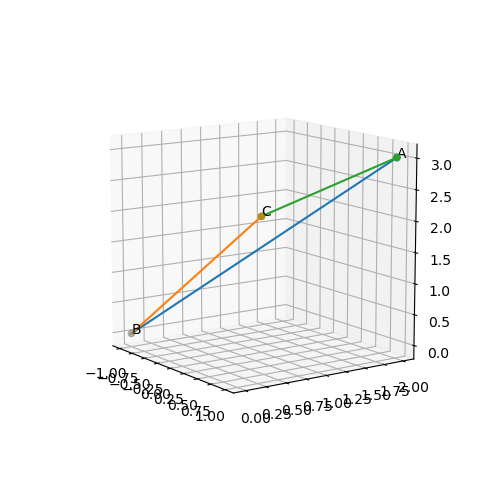
\includegraphics[width=\columnwidth]{chapters/12/10/3/15/figs/Figure_1.png}
   \caption{}
   \label{fig:chapters/12/10/3/15/TriangleABC}
\end{figure}





    \item Find the direction cosines of a line which makes equal angles with the coordinate
    axes.
		\\
		\solution
		\iffalse
\documentclass[journal,12pt,twocolumn]{IEEEtran}
\usepackage{setspace}
\usepackage{gensymb}
\usepackage{xcolor}
\usepackage{caption}
\singlespacing
\usepackage{siunitx}
\usepackage[cmex10]{amsmath}
\usepackage{mathtools}
\usepackage{hyperref}
\usepackage{amsthm}
\usepackage{mathrsfs}
\usepackage{txfonts}
\usepackage{stfloats}
\usepackage{cite}
\usepackage{cases}
\usepackage{subfig}
\usepackage{longtable}
\usepackage{multirow}
\usepackage{enumitem}
\usepackage{bm}
\usepackage{mathtools}
\usepackage{listings}
\usepackage{tikz}
\usetikzlibrary{shapes,arrows,positioning}
\usepackage{circuitikz}
\renewcommand{\vec}[1]{\boldsymbol{\mathbf{#1}}}
\DeclareMathOperator*{\Res}{Res}
\renewcommand\thesection{\arabic{section}}
\renewcommand\thesubsection{\thesection.\arabic{subsection}}
\renewcommand\thesubsubsection{\thesubsection.\arabic{subsubsection}}

\renewcommand\thesectiondis{\arabic{section}}
\renewcommand\thesubsectiondis{\thesectiondis.\arabic{subsection}}
\renewcommand\thesubsubsectiondis{\thesubsectiondis.\arabic{subsubsection}}
\hyphenation{op-tical net-works semi-conduc-tor}

\lstset{
language=Python,
frame=single, 
breaklines=true,
columns=fullflexible
}
\begin{document}
\theoremstyle{definition}
\newtheorem{theorem}{Theorem}[section]
\newtheorem{problem}{Problem}
\newtheorem{proposition}{Proposition}[section]
\newtheorem{lemma}{Lemma}[section]
\newtheorem{corollary}[theorem]{Corollary}
\newtheorem{example}{Example}[section]
\newtheorem{definition}{Definition}[section]
\newcommand{\BEQA}{\begin{eqnarray}}
\newcommand{\EEQA}{\end{eqnarray}}
\newcommand{\define}{\stackrel{\triangle}{=}}
\newcommand{\myvec}[1]{\ensuremath{\begin{pmatrix}#1\end{pmatrix}}}
\newcommand{\mydet}[1]{\ensuremath{\begin{vmatrix}#1\end{vmatrix}}}
\bibliographystyle{IEEEtran}
\providecommand{\nCr}[2]{\,^{#1}C_{#2}} % nCr
\providecommand{\nPr}[2]{\,^{#1}P_{#2}} % nPr
\providecommand{\mbf}{\mathbf}
\providecommand{\pr}[1]{\ensuremath{\Pr\left(#1\right)}}
\providecommand{\qfunc}[1]{\ensuremath{Q\left(#1\right)}}
\providecommand{\sbrak}[1]{\ensuremath{{}\left[#1\right]}}
\providecommand{\lsbrak}[1]{\ensuremath{{}\left[#1\right.}}
\providecommand{\rsbrak}[1]{\ensuremath{{}\left.#1\right]}}
\providecommand{\brak}[1]{\ensuremath{\left(#1\right)}}
\providecommand{\lbrak}[1]{\ensuremath{\left(#1\right.}}
\providecommand{\rbrak}[1]{\ensuremath{\left.#1\right)}}
\providecommand{\cbrak}[1]{\ensuremath{\left\{#1\right\}}}
\providecommand{\lcbrak}[1]{\ensuremath{\left\{#1\right.}}
\providecommand{\rcbrak}[1]{\ensuremath{\left.#1\right\}}}
\theoremstyle{remark}
\newtheorem{rem}{Remark}
\newcommand{\sgn}{\mathop{\mathrm{sgn}}}
\newcommand{\rect}{\mathop{\mathrm{rect}}}
\newcommand{\sinc}{\mathop{\mathrm{sinc}}}
\providecommand{\abs}[1]{\left\vert#1\right\vert}
\providecommand{\res}[1]{\Res\displaylimits_{#1}} 
\providecommand{\norm}[1]{\lVert#1\rVert}
\providecommand{\mtx}[1]{\mathbf{#1}}
\providecommand{\mean}[1]{E\left[ #1 \right]}
\providecommand{\fourier}{\overset{\mathcal{F}}{ \rightleftharpoons}}
\providecommand{\ztrans}{\overset{\mathcal{Z}}{ \rightleftharpoons}}
\providecommand{\system}[1]{\overset{\mathcal{#1}}{ \longleftrightarrow}}
\newcommand{\solution}{\noindent \textbf{Solution: }}
\providecommand{\dec}[2]{\ensuremath{\overset{#1}{\underset{#2}{\gtrless}}}}
\let\StandardTheFigure\thefigure
\def\putbox#1#2#3{\makebox[0in][l]{\makebox[#1][l]{}\raisebox{\baselineskip}[0in][0in]{\raisebox{#2}[0in][0in]{#3}}}}
     \def\rightbox#1{\makebox[0in][r]{#1}}
     \def\centbox#1{\makebox[0in]{#1}}
     \def\topbox#1{\raisebox{-\baselineskip}[0in][0in]{#1}}
     \def\midbox#1{\raisebox{-0.5\baselineskip}[0in][0in]{#1}}

\vspace{3cm}
\title{12.11.1.2}
\author{Lokesh Surana}
\maketitle
\section*{Class 12, Chapter 11, Exercise 1.2}

\begin{enumerate}[start=2]

    \solution 
\fi
The unit direction vector can be expressed as
    \begin{align}
	    \vec{x} &= \myvec{\cos\alpha\\\cos\alpha\\\cos\alpha} 
	\\
	\implies
	    \norm{\vec{x}} &= 
       \cos\alpha \sqrt{3} = 1
\implies        \cos\alpha = \pm\frac{1}{\sqrt{3}}
    \end{align}
    Thus
    \begin{align}
	    \vec{x} = \pm\frac{1}{\sqrt{3}} \myvec{1 \\ 1 \\ 1} 
\end{align}
    

\item Find a unit vector perpendicular to each of the vector $\overrightarrow{a}+\overrightarrow{b}\text{ and }\overrightarrow{a}-\overrightarrow{b},\text{ where } \overrightarrow{a}=3\hat{i}+2\hat{j}+2\hat{k}\text{ and } \overrightarrow{b}=\hat{i}+2\hat{j}-2\hat{k}$. 
	\\
		\solution
		\iffalse
\documentclass[12pt]{article}
\usepackage{graphicx}
\usepackage[none]{hyphenat}
\usepackage{graphicx}
\usepackage{listings}
\usepackage[english]{babel}
\usepackage{graphicx}
\usepackage{caption} 
\usepackage{booktabs}
\usepackage{array}
\usepackage{amssymb} % for \because
\usepackage{amsmath}   % for having text in math mode
\usepackage{extarrows} % for Row operations arrows
\usepackage{listings}
\usepackage[utf8]{inputenc}
\lstset{
  frame=single,
  breaklines=true
}
\usepackage{hyperref}
  
%Following 2 lines were added to remove the blank page at the beginning
\usepackage{atbegshi}% http://ctan.org/pkg/atbegshi
\AtBeginDocument{\AtBeginShipoutNext{\AtBeginShipoutDiscard}}


%New macro definitions
\newcommand{\mydet}[1]{\ensuremath{\begin{vmatrix}#1\end{vmatrix}}}
\providecommand{\brak}[1]{\ensuremath{\left(#1\right)}}
\newcommand{\solution}{\noindent \textbf{Solution: }}
\newcommand{\myvec}[1]{\ensuremath{\begin{pmatrix}#1\end{pmatrix}}}
\providecommand{\norm}[1]{\left\lVert#1\right\rVert}
\providecommand{\abs}[1]{\left\vert#1\right\vert}
\let\vec\mathbf
\begin{document}
\begin{center}
\title{\textbf{  Unit Vector Perpendicular}}
\date{\vspace{-5ex}} %Not to print date automatically
\maketitle
\end{center}
\setcounter{page}{1}
\section{12$^{th}$ Maths - Chapter 10}
\textbf{This is Problem-2 from Exercise 10.4}
\begin{enumerate}

\item Find a unit vector  perpendicular to each of a vector $\bar{a}+\bar{b} \text{ and }\bar{a}-\bar{b}$ where  $\overrightarrow{a}=3\hat{i}+2\hat{j}+2\hat{k}\text{ and }\overrightarrow{b}=\hat{i}+2\hat{j}-2\hat{k}$
\section{Solution}
\fi
Since
\begin{align}
	\vec{a}+\vec{b}=\myvec{4\\4\\0},\,
	\vec{a}-\vec{b}=\myvec{2\\0\\4}
\end{align}
the desired vector is obtained as
\begin{align} 
\myvec{\vec{a}+\vec{b}& \vec{a}-\vec{b}}^\top\vec{x}=0\\
\implies
\myvec{
4&4&0\\
2&0&4
}
\xleftrightarrow[]{R_1=\frac{R_1}{4}}
\myvec{
1&1&0\\
2&0&4
}\xleftrightarrow[]{R_2=\frac{R_2}{2}}
\myvec{
1&1&0\\
1&0&2
}\\
\xleftrightarrow[]{R_2={R_1}-{R_2}}
\myvec{
1&1&0\\
0&-1&2
}
\xleftrightarrow[]{R_2=\frac{R_2}{-1}}
\myvec{
1&1&0\\
0&1&-2
}
\xleftrightarrow[]{R_1={R_1}-{R_2}}
\myvec{
1&0&2\\
0&1&-2
}
\end{align}
yielding
\begin{align}
\begin{split}
x_1+2x_3=0\\
x_2-2x_3=0
\end{split}
\implies 
\vec{x}
=x_3\myvec{-2\\2\\1}
\end{align}

\item If a unit vector $\overrightarrow{a}$ makes angles $\dfrac{\pi}{3}\text{ with }\hat{i}, \dfrac{\pi}{4}\text{ with }\hat{j}$ and an acute angle $\theta \text{ with }\hat{k},\text{ then find } \theta$ and hence, the components of $\overrightarrow{a}$.
	\\
		\solution
		\iffalse
\documentclass[12pt]{article}
\usepackage{graphicx}
%\documentclass[journal,12pt,twocolumn]{IEEEtran}
\usepackage[none]{hyphenat}
\usepackage{graphicx}
\usepackage{listings}
\usepackage[english]{babel}
\usepackage{graphicx}
\usepackage{caption}
\usepackage[parfill]{parskip}
\usepackage{hyperref}
\usepackage{booktabs}
\usepackage{gensymb}
%\usepackage{setspace}\doublespacing\pagestyle{plain}
\def\inputGnumericTable{}
\usepackage{color}                                            %%
    \usepackage{array}                                            %%
    \usepackage{longtable}                                        %%
    \usepackage{calc}                                             %%
    \usepackage{multirow}                                         %%
    \usepackage{hhline}                                           %%
    \usepackage{ifthen}
\usepackage{array}
\usepackage{amsmath}   % for having text in math mode
\usepackage{parallel,enumitem}
\usepackage{listings}
\lstset{
language=tex,
frame=single,
breaklines=true
}
 
%Following 2 lines were added to remove the blank page at the beginning
\usepackage{atbegshi}% http://ctan.org/pkg/atbegshi
\AtBeginDocument{\AtBeginShipoutNext{\AtBeginShipoutDiscard}}
%
%New macro definitions
\newcommand{\mydet}[1]{\ensuremath{\begin{vmatrix}#1\end{vmatrix}}}
\providecommand{\brak}[1]{\ensuremath{\left(#1\right)}}
\providecommand{\norm}[1]{\left\lVert#1\right\rVert}
\newcommand{\solution}{\noindent \textbf{Solution: }}
\newcommand{\myvec}[1]{\ensuremath{\begin{pmatrix}#1\end{pmatrix}}}
\let\vec\mathbf
\begin{document}
\begin{center}
\enlargethispage{-4cm}
\title{\textbf{Vector Algebra}}
\date{\vspace{-5ex}} %Not to print date automatically
\maketitle
\end{center}
\setcounter{page}{1}
\section*{12$^{th}$ Maths - Chapter 10}
This is Problem-3 from Exercise 10.4
\begin{enumerate}
\item If unit vector $\overrightarrow{a}$ makes angles $\frac{\pi}{3}$ with $\hat{i}$, $\frac{\pi}{4}$ with $\hat{j}$ and an acute angle $\theta$ with $\hat{k}$, then find $\theta$ and hence, the components of $\overrightarrow{a}$.

\solution
\fi
		Let 
		\begin{align}
			\vec{A}=\myvec{\cos\theta_1\\\cos\theta_2\\\cos\theta_3}
		\end{align}
		where
		\begin{align}
		\cos\theta_1 &=\cos\frac{\pi}{3}
			=\frac{1}{2}\\
			\cos\theta_2 &=\cos\frac{\pi}{4}\\
			=\frac{1}{\sqrt{2}}
		\end{align}
		Since
\begin{align}
    \norm{\vec{A}}&=1,
\sqrt{\cos^2\theta_1+\cos^2\theta_2+\cos^2\theta_3}&=1
    \implies\sqrt{\frac{1}{2}^2+\frac{1}{\sqrt{2}}^2+\cos^2\theta_3 }&=1\\
    \implies\cos\theta_3 &=\pm\frac{1}{2}
\end{align}
Since $\theta_3$ is an acute angle
\begin{align}
 \cos\theta_3=\frac{1}{2}
\end{align}
    Hence 
\begin{align}
		\vec{A}=\myvec{\frac{1}{2}\\[2pt] \frac{1}{\sqrt{2}}\\[2pt] \frac{1}{2}}
\end{align}

\item Show that the direction cosines of a vector equally inclined to the axes OX, OY and OZ are \textpm $\sbrak{\frac{1}{\sqrt{3}},\frac{1}{\sqrt{3}},\frac{1}{\sqrt{3}}}$.\\
	\solution
		\iffalse
\documentclass[journal,12pt,twocolumn]{IEEEtran}
%
\usepackage{setspace}
\usepackage{gensymb}
%\doublespacing
\singlespacing

%\usepackage{graphicx}
%\usepackage{amssymb}
%\usepackage{relsize}
\usepackage[cmex10]{amsmath}
%\usepackage{amsthm}
%\interdisplaylinepenalty=2500
%\savesymbol{iint}
%\usepackage{txfonts}
%\restoresymbol{TXF}{iint}
%\usepackage{wasysym}
\usepackage{amsthm}
%\usepackage{iithtlc}
\usepackage{mathrsfs}
\usepackage{txfonts}
\usepackage{stfloats}
\usepackage{bm}
\usepackage{cite}
\usepackage{cases}
\usepackage{subfig}
%\usepackage{xtab}
\usepackage{longtable}
\usepackage{multirow}
%\usepackage{algorithm}
%\usepackage{algpseudocode}
\usepackage{enumitem}
\usepackage{mathtools}
\usepackage{steinmetz}
\usepackage{tikz}
\usepackage{circuitikz}
\usepackage{verbatim}
\usepackage{tfrupee}
\usepackage[breaklinks=true]{hyperref}
%\usepackage{stmaryrd}
\usepackage{tkz-euclide} % loads  TikZ and tkz-base
%\usetkzobj{all}
\usetikzlibrary{calc,math}
\usepackage{listings}
    \usepackage{color}                                            %%
    \usepackage{array}                                            %%
    \usepackage{longtable}                                        %%
    \usepackage{calc}                                             %%
    \usepackage{multirow}                                         %%
    \usepackage{hhline}                                           %%
    \usepackage{ifthen}                                           %%
  %optionally (for landscape tables embedded in another document): %%
    \usepackage{lscape}     
\usepackage{multicol}
\usepackage{chngcntr}
%\usepackage{enumerate}

%\usepackage{wasysym}
%\newcounter{MYtempeqncnt}
\DeclareMathOperator*{\Res}{Res}
%\renewcommand{\baselinestretch}{2}
\renewcommand\thesection{\arabic{section}}
\renewcommand\thesubsection{\thesection.\arabic{subsection}}
\renewcommand\thesubsubsection{\thesubsection.\arabic{subsubsection}}

\renewcommand\thesectiondis{\arabic{section}}
\renewcommand\thesubsectiondis{\thesectiondis.\arabic{subsection}}
\renewcommand\thesubsubsectiondis{\thesubsectiondis.\arabic{subsubsection}}

% correct bad hyphenation here
\hyphenation{op-tical net-works semi-conduc-tor}
\def\inputGnumericTable{}                                 %%

\lstset{
%language=C,
frame=single, 
breaklines=true,
columns=fullflexible
}
%\lstset{
%language=tex,
%frame=single, 
%breaklines=true
%}

\begin{document}
%


\newtheorem{theorem}{Theorem}[section]
\newtheorem{problem}{Problem}
\newtheorem{proposition}{Proposition}[section]
\newtheorem{lemma}{Lemma}[section]
\newtheorem{corollary}[theorem]{Corollary}
\newtheorem{example}{Example}[section]
\newtheorem{definition}[problem]{Definition}
%\newtheorem{thm}{Theorem}[section] 
%\newtheorem{defn}[thm]{Definition}
%\newtheorem{algorithm}{Algorithm}[section]
%\newtheorem{cor}{Corollary}
\newcommand{\BEQA}{\begin{eqnarray}}
\newcommand{\EEQA}{\end{eqnarray}}
\newcommand{\define}{\stackrel{\triangle}{=}}

\bibliographystyle{IEEEtran}
%\bibliographystyle{ieeetr}


\providecommand{\mbf}{\mathbf}
\providecommand{\pr}[1]{\ensuremath{\Pr\left(#1\right)}}
\providecommand{\qfunc}[1]{\ensuremath{Q\left(#1\right)}}
\providecommand{\sbrak}[1]{\ensuremath{{}\left[#1\right]}}
\providecommand{\lsbrak}[1]{\ensuremath{{}\left[#1\right.}}
\providecommand{\rsbrak}[1]{\ensuremath{{}\left.#1\right]}}
\providecommand{\brak}[1]{\ensuremath{\left(#1\right)}}
\providecommand{\lbrak}[1]{\ensuremath{\left(#1\right.}}
\providecommand{\rbrak}[1]{\ensuremath{\left.#1\right)}}
\providecommand{\cbrak}[1]{\ensuremath{\left\{#1\right\}}}
\providecommand{\lcbrak}[1]{\ensuremath{\left\{#1\right.}}
\providecommand{\rcbrak}[1]{\ensuremath{\left.#1\right\}}}
\theoremstyle{remark}
\newtheorem{rem}{Remark}
\newcommand{\sgn}{\mathop{\mathrm{sgn}}}
\providecommand{\abs}[1]{\left\vert#1\right\vert}
\providecommand{\res}[1]{\Res\displaylimits_{#1}} 
\providecommand{\norm}[1]{\left\lVert#1\right\rVert}
%\providecommand{\norm}[1]{\lVert#1\rVert}
\providecommand{\mtx}[1]{\mathbf{#1}}
\providecommand{\mean}[1]{E\left[ #1 \right]}
\providecommand{\fourier}{\overset{\mathcal{F}}{ \rightleftharpoons}}
%\providecommand{\hilbert}{\overset{\mathcal{H}}{ \rightleftharpoons}}
\providecommand{\system}{\overset{\mathcal{H}}{ \longleftrightarrow}}
	%\newcommand{\solution}[2]{\textbf{Solution:}{#1}}
\newcommand{\solution}{\noindent \textbf{Solution: }}
\newcommand{\cosec}{\,\text{cosec}\,}
\providecommand{\dec}[2]{\ensuremath{\overset{#1}{\underset{#2}{\gtrless}}}}
\newcommand{\myvec}[1]{\ensuremath{\begin{pmatrix}#1\end{pmatrix}}}
\newcommand{\mydet}[1]{\ensuremath{\begin{vmatrix}#1\end{vmatrix}}}
%\numberwithin{equation}{section}
\numberwithin{equation}{subsection}
%\numberwithin{problem}{section}
%\numberwithin{definition}{section}
\makeatletter
\@addtoreset{figure}{problem}
\makeatother

\let\StandardTheFigure\thefigure
\let\vec\mathbf
%\renewcommand{\thefigure}{\theproblem.\arabic{figure}}
\renewcommand{\thefigure}{\theproblem}
%\setlist[enumerate,1]{before=\renewcommand\theequation{\theenumi.\arabic{equation}}
%\counterwithin{equation}{enumi}


%\renewcommand{\theequation}{\arabic{subsection}.\arabic{equation}}

\def\putbox#1#2#3{\makebox[0in][l]{\makebox[#1][l]{}\raisebox{\baselineskip}[0in][0in]{\raisebox{#2}[0in][0in]{#3}}}}
     \def\rightbox#1{\makebox[0in][r]{#1}}
     \def\centbox#1{\makebox[0in]{#1}}
     \def\topbox#1{\raisebox{-\baselineskip}[0in][0in]{#1}}
     \def\midbox#1{\raisebox{-0.5\baselineskip}[0in][0in]{#1}}

\vspace{3cm}


\title{Question: 12.10.5.11}
\author{Nikam Pratik Balasaheb (EE21BTECH11037)}





% make the title area
\maketitle

\newpage

%\tableofcontents

\bigskip

\renewcommand{\thefigure}{\theenumi}
\renewcommand{\thetable}{\theenumi}
%\renewcommand{\theequation}{\theenumi}

\section{Problem}
Show that direction cosines of a vector equally inclined to axes $ \vec{OX}, \vec{OY}$ and $\vec{OZ}$ are $\pm \myvec{\frac{1}{\sqrt{3}} \\[1pt] \frac{1}{\sqrt{3}} \\[1pt] \frac{1}{\sqrt{3}}} $
\section{Solution}
The vector is equally inclined to the axes $\vec{OX}$, $\vec{OY}$ and $\vec{OZ}$. Let the angle be $\theta$.
\fi

The direction vector can be expressed in terms of the direction cosines as 
\begin{align}
\vec{m}  = \myvec{\cos{\theta} \\ \cos{\theta} \\ \cos{\theta} }
\end{align}
Since 
\begin{align}
\norm{\vec{m}} = 1,
\abs{\sqrt{3} \cos{\theta}} =1 \implies
\cos{\theta} = \pm \frac{1}{\sqrt{3}}
\end{align}


\item Write down a unit vector in XY-plane, making an angle of 30$^{\circ}$ with the positive direction of x-axis.\\
\item The scalar product of the vector $\hat{i}+\hat{j}+\hat{k}$ with a unit vector along the sum of vectors $2\hat{i}+4\hat{j}-5\hat{k}$ and $\lambda\hat{i}+2\hat{j}+3\hat{k}$ is equal to one. Find the value of $\lambda$.
\item If $\theta$ is the angle between two vectors $\vec{a}$ and $\vec{b}$,then $\vec{a}.\vec{b}\geq0$ only when 
\begin{enumerate}
\item \label{itm:chapters/12/10/5/161} $0<\theta<\frac{\pi}{2}$
\item \label{itm:chapters/12/10/5/162} $0\le\theta\le\frac{\pi}{2}$
\item \label{itm:chapters/12/10/5/163} $0<\theta<\pi$
\item \label{itm:chapters/12/10/5/164} $0\le\theta\le\pi$
\end{enumerate}
	\solution
		\iffalse
\documentclass[10pt]{article}
\usepackage{graphicx}
\usepackage[none]{hyphenat}
\usepackage{listings}
\usepackage[english]{babel}
\usepackage{siunitx}
\usepackage{caption}
\usepackage{booktabs}
\usepackage{array}
\usepackage{extarrows}
\usepackage{enumerate}
\usepackage{enumitem}
\usepackage{amsmath}
\usepackage{commath}
\usepackage{gensymb}
\usepackage{amssymb}
\usepackage{multicol}
\usepackage[utf8]{inputenc}
\lstset{
 frame=single,
 breaklines=true
}
\usepackage{hyperref}
\usepackage[margin=0.8in]{geometry}
%\usepackage{exsheets}% also loads the `tasks' package
\usepackage{atbegshi}
\AtBeginDocument{\AtBeginShipoutNext{\AtBeginShipoutDiscard}}

%new macro definitions
\renewcommand{\labelenumi}{(\alph{enumi})}
\newcommand{\mydet}[1]{\ensuremath{\begin{vmatrix}#1\end{vmatrix}}}
\providecommand{\brak}[1]{\ensuremath{\left(#1\right)}}
\newcommand{\solution}{\noindent \textbf{Solution: }}
\newcommand{\myvec}[1]{\ensuremath{\begin{pmatrix}#1\end{pmatrix}}}
\providecommand{\norm}[1]{\left\1Vert#1\right\rVert}
\let\vec\mathbf{}


%\SetEnumitemKey{twocol}{
% before=\raggedcolumns\begin{multicols}{2},
% after=\end{multicols}}
%\SetEnumitemKey{fourcol}{
% before=\raggedcolumns\begin{multicols}{4},
% after=\end{multicols}} 


\begin{document}
\begin{center}
\title{\textbf{VECTORS}}
\date{\vspace{-5ex}}
\maketitle
\end{center}
\section*{12$^{th}$Math - Chapter 10}
This is Problem-16 from Exercise 10.5\\\\
If $\theta$ is the angle between two vectors $\overrightarrow{\vec{a}}$ and $\overrightarrow{\vec{b}}$,then$\overrightarrow{\vec{a}}\cdot\overrightarrow{\vec{b}}\ge 0$ only when
\begin{enumerate}[ref=(\alph*)]
\end{enumerate}
\solution
\fi
Since
\begin{align}
 {\vec{a}^{\top}\vec{b}}&=\cos\theta\norm{\vec{a}}\norm{\vec{b}},\\
 {\vec{a}^{\top}\vec{b}}&\ge0 \implies 
 \cos\theta\ge0\\
	\therefore 0\le\theta\le\frac{\pi}{2},& \frac{3\pi}{2}\le\theta\le{2\pi}.
\label{eq:chapters/12/10/5/161}
\end{align}
\begin{enumerate}
\item $0<\theta<\frac{\pi}{2}$:
Comparing with \eqref{eq:chapters/12/10/5/161}, option \ref{itm:chapters/12/10/5/161} is incorrect.
\item $0\le\theta\le\frac{\pi}{2}$:
Comparing with \eqref{eq:chapters/12/10/5/161}, option \ref{itm:chapters/12/10/5/162} is correct.
\item $0<\theta<\pi$:
Comparing with \eqref{eq:chapters/12/10/5/161}, option \ref{itm:chapters/12/10/5/163} is incorrect.
\item $0\le\theta\le\pi$:
Comparing with \eqref{eq:chapters/12/10/5/161}, option \ref{itm:chapters/12/10/5/164} is incorrect.
\end{enumerate}

\item Find the slope of the line, which makes an angle of 30 degrees with the positive direction of y-axis measures anticlockwise.
\label{chapters/11/10/1/7}\\
\solution
\iffalse
\documentclass[journal,12pt,twocolumn]{IEEEtran}
%
\usepackage{setspace}
\usepackage{gensymb}
%\doublespacing
\singlespacing

%\usepackage{graphicx}
%\usepackage{amssymb}
%\usepackage{relsize}
\usepackage[cmex10]{amsmath}
%\usepackage{amsthm}
%\interdisplaylinepenalty=2500
%\savesymbol{iint}
%\usepackage{txfonts}
%\restoresymbol{TXF}{iint}
%\usepackage{wasysym}
\usepackage{amsthm}
%\usepackage{iithtlc}
\usepackage{mathrsfs}
\usepackage{txfonts}
\usepackage{stfloats}
\usepackage{bm}
\usepackage{cite}
\usepackage{cases}
\usepackage{subfig}
%\usepackage{xtab}
\usepackage{longtable}
\usepackage{multirow}
%\usepackage{algorithm}
%\usepackage{algpseudocode}
\usepackage{enumitem}
\usepackage{mathtools}
\usepackage{steinmetz}
\usepackage{tikz}
\usepackage{circuitikz}
\usepackage{verbatim}
\usepackage{tfrupee}
\usepackage[breaklinks=true]{hyperref}
%\usepackage{stmaryrd}
\usepackage{tkz-euclide} % loads  TikZ and tkz-base
%\usetkzobj{all}
\usetikzlibrary{calc,math}
\usepackage{listings}
    \usepackage{color}                                            %%
    \usepackage{array}                                            %%
    \usepackage{longtable}                                        %%
    \usepackage{calc}                                             %%
    \usepackage{multirow}                                         %%
    \usepackage{hhline}                                           %%
    \usepackage{ifthen}                                           %%
  %optionally (for landscape tables embedded in another document): %%
    \usepackage{lscape}     
\usepackage{multicol}
\usepackage{chngcntr}
%\usepackage{enumerate}

%\usepackage{wasysym}
%\newcounter{MYtempeqncnt}
\DeclareMathOperator*{\Res}{Res}
%\renewcommand{\baselinestretch}{2}
\renewcommand\thesection{\arabic{section}}
\renewcommand\thesubsection{\thesection.\arabic{subsection}}
\renewcommand\thesubsubsection{\thesubsection.\arabic{subsubsection}}

\renewcommand\thesectiondis{\arabic{section}}
\renewcommand\thesubsectiondis{\thesectiondis.\arabic{subsection}}
\renewcommand\thesubsubsectiondis{\thesubsectiondis.\arabic{subsubsection}}

% correct bad hyphenation here
\hyphenation{op-tical net-works semi-conduc-tor}
\def\inputGnumericTable{}                                 %%

\lstset{
%language=C,
frame=single, 
breaklines=true,
columns=fullflexible
}
%\lstset{
%language=tex,
%frame=single, 
%breaklines=true
%}


\begin{document}
%


\newtheorem{theorem}{Theorem}[section]
\newtheorem{problem}{Problem}
\newtheorem{proposition}{Proposition}[section]
\newtheorem{lemma}{Lemma}[section]
\newtheorem{corollary}[theorem]{Corollary}
\newtheorem{example}{Example}[section]
\newtheorem{definition}[problem]{Definition}
%\newtheorem{thm}{Theorem}[section] 
%\newtheorem{defn}[thm]{Definition}
%\newtheorem{algorithm}{Algorithm}[section]
%\newtheorem{cor}{Corollary}
\newcommand{\BEQA}{\begin{eqnarray}}
\newcommand{\EEQA}{\end{eqnarray}}
\newcommand{\define}{\stackrel{\triangle}{=}}

\bibliographystyle{IEEEtran}
%\bibliographystyle{ieeetr}


\providecommand{\mbf}{\mathbf}
\providecommand{\pr}[1]{\ensuremath{\Pr\left(#1\right)}}
\providecommand{\qfunc}[1]{\ensuremath{Q\left(#1\right)}}
\providecommand{\sbrak}[1]{\ensuremath{{}\left[#1\right]}}
\providecommand{\lsbrak}[1]{\ensuremath{{}\left[#1\right.}}
\providecommand{\rsbrak}[1]{\ensuremath{{}\left.#1\right]}}
\providecommand{\brak}[1]{\ensuremath{\left(#1\right)}}
\providecommand{\lbrak}[1]{\ensuremath{\left(#1\right.}}
\providecommand{\rbrak}[1]{\ensuremath{\left.#1\right)}}
\providecommand{\cbrak}[1]{\ensuremath{\left\{#1\right\}}}
\providecommand{\lcbrak}[1]{\ensuremath{\left\{#1\right.}}
\providecommand{\rcbrak}[1]{\ensuremath{\left.#1\right\}}}
\theoremstyle{remark}
\newtheorem{rem}{Remark}
\newcommand{\sgn}{\mathop{\mathrm{sgn}}}
\providecommand{\abs}[1]{\left\vert#1\right\vert}
\providecommand{\res}[1]{\Res\displaylimits_{#1}} 
\providecommand{\norm}[1]{\left\lVert#1\right\rVert}
%\providecommand{\norm}[1]{\lVert#1\rVert}
\providecommand{\mtx}[1]{\mathbf{#1}}
\providecommand{\mean}[1]{E\left[ #1 \right]}
\providecommand{\fourier}{\overset{\mathcal{F}}{ \rightleftharpoons}}
%\providecommand{\hilbert}{\overset{\mathcal{H}}{ \rightleftharpoons}}
\providecommand{\system}{\overset{\mathcal{H}}{ \longleftrightarrow}}
	%\newcommand{\solution}[2]{\textbf{Solution:}{#1}}
\newcommand{\solution}{\noindent \textbf{Solution: }}
\newcommand{\cosec}{\,\text{cosec}\,}
\providecommand{\dec}[2]{\ensuremath{\overset{#1}{\underset{#2}{\gtrless}}}}
\newcommand{\myvec}[1]{\ensuremath{\begin{pmatrix}#1\end{pmatrix}}}
\newcommand{\mydet}[1]{\ensuremath{\begin{vmatrix}#1\end{vmatrix}}}
%\numberwithin{equation}{section}
\numberwithin{equation}{subsection}
%\numberwithin{problem}{section}
%\numberwithin{definition}{section}
\makeatletter
\@addtoreset{figure}{problem}
\makeatother

\let\StandardTheFigure\thefigure
\let\vec\mathbf
%\renewcommand{\thefigure}{\theproblem.\arabic{figure}}
\renewcommand{\thefigure}{\theproblem}
%\setlist[enumerate,1]{before=\renewcommand\theequation{\theenumi.\arabic{equation}}
%\counterwithin{equation}{enumi}


%\renewcommand{\theequation}{\arabic{subsection}.\arabic{equation}}

\def\putbox#1#2#3{\makebox[0in][l]{\makebox[#1][l]{}\raisebox{\baselineskip}[0in][0in]{\raisebox{#2}[0in][0in]{#3}}}}
     \def\rightbox#1{\makebox[0in][r]{#1}}
     \def\centbox#1{\makebox[0in]{#1}}
     \def\topbox#1{\raisebox{-\baselineskip}[0in][0in]{#1}}
     \def\midbox#1{\raisebox{-0.5\baselineskip}[0in][0in]{#1}}

\vspace{3cm}


\title{Quiz 4}
\author{S Nithish}





% make the title area
\maketitle

\newpage

%\tableofcontents

\bigskip

\renewcommand{\thefigure}{\theenumi}
\renewcommand{\thetable}{\theenumi}
%\renewcommand{\theequation}{\theenumi}


\begin{abstract}
This document contains the solution of the question from NCERT 11th standard chapter 10 exercise 10.1 problem 7
\end{abstract}

%Download all python codes 
%
%\begin{lstlisting}
%svn co https://github.com/JayatiD93/trunk/My_solution_design/codes
%\end{lstlisting}

%Download all and latex-tikz codes from 
%
%\begin{lstlisting}
%svn co https://github.com/gadepall/school/trunk/ncert/geometry/figs
%\end{lstlisting}
%


\section{Exercise 10.1}

\begin{enumerate}

	\fi
Let the direction vector of the y-axis be
\begin{align}
\vec{m_1} = \myvec{0 \\ 1}
\end{align}
and the direction vector of the line be,
\begin{align}
\vec{m_2} = \myvec{1 \\ m}
\end{align}
where $m$ is the slope of the line.
Then, 
\begin{align}
	\vec{m_1}^{\top} \vec{m_2}   = m, \,
	\norm{\vec{m_1}}   = 1, \,
	\norm{\vec{m_2}}  = \sqrt{1+m^2}
\end{align}
yielding
the angle between the two as
\begin{align}
	\cos (\phi) &= \frac{m}{\sqrt{1+m^2}}
	 = \frac{\sqrt{3}}{2}\\
\implies
	m &= \pm \sqrt{3} 
\end{align}
Thus, 
$m=\sqrt{3}$ is the correct slope.


\item Find the angle between x-axis and the line joining points (3,-1) and (4,-2).
\label{chapters/11/10/1/10}
\iffalse
\def\mytitle{PYTHON PROGRAMMING ON MATRICES}
\def\myauthor{Revathi pamujula}
\def\contact{revathipamujula111@gmail.com}
\def\mymodule{Future Wireless Communication (FWC)}


\documentclass[10pt, a4paper]{article}
\usepackage[a4paper,outer=1.5cm,inner=1.5cm,top=1.75cm,bottom=1.5cm]{geometry}

\twocolumn
\usepackage{graphicx}
%\usepackage{karnaugh-map}
\usepackage{tabularx}
\usepackage{hyperref}
\usepackage[utf8]{inputenc}
\usepackage{amsmath}
%\usepackage{physics}
\usepackage{amssymb}
\usepackage{watermark}
\renewcommand*\familydefault{\sfdefault}
\usepackage{lipsum}
\usepackage{xcolor}
\usepackage{listings}
\let\vec\mathbf
\lstset{
frame=single, 
breaklines=true,
columns=fullflexible
}

\begin{document}
\title{\mytitle}
\author{\myauthor\hspace{1em}\\\contact\\FWC22045\hspace{6.5em}IITH\hspace{0.5em}\mymodule\hspace{6em}Matrix:Lines}

%\{ Wireless Communication (FWC)}
\date{}
\maketitle


  \section{Problem}
  \fi
\\
\solution See Fig. 
		\ref{fig:11/10/1/10}.
	\begin{figure}[!ht]
		\centering
 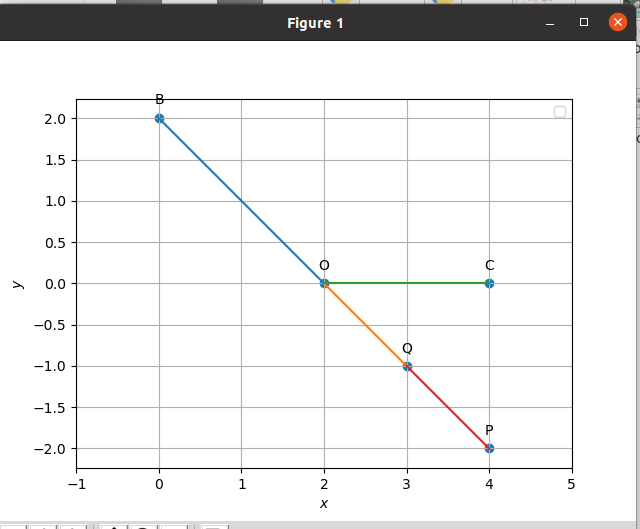
\includegraphics[width=\columnwidth]{chapters/11/10/1/10/figs/fig.png}
		\caption{}
		\label{fig:11/10/1/10}
  	\end{figure}

	\iffalse
\section{Solution}
\textbf{Given that:}
\begin{center}

%\boldmath
	\fi
	Let 
\begin{align}
\vec{P}=\myvec{ 3\\ -1 },
\vec{Q}=\myvec{ 4\\ -2 }
\end{align}
Then 
\begin{align}
	\vec{C}=\vec{P}-\vec{Q}
=\myvec{ -1\\ 1 }
\end{align}
The desired angle is given by
\begin{align}
	\cos\theta&=\frac{\vec{C}^{T}\vec{e}_1}{\norm{\vec{C}}\norm{\vec{e}_1}}
	\\
	&= -\frac{1}{\sqrt{2}}
	\\
	\implies 
	\theta&=135\degree
 \end{align}
 \iffalse
\begin{figure}[h!]
  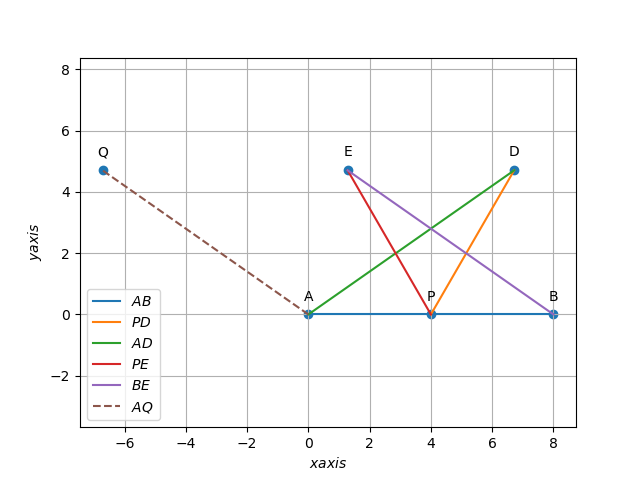
\includegraphics[scale=0.5]{fig.png}
  \caption{line assignment }
  \label{fig:line assignment}
\end{figure}
\end{document}
\fi

	\item The slope of a line is double of the slope of another line. If tangent of the angle between them is 1/3, find the slopes of the lines.
\label{chapters/11/10/1/11}
\iffalse
\documentclass[10pt,a4paper]{report}
%\usepackage[latin1]{inputenc}
\usepackage[utf8]{inputenc}
\usepackage{amsmath}
\usepackage{amsfonts}
\usepackage{amssymb}
\usepackage{graphicx}
\usepackage{multicol}
\usepackage{tabularx}
\usepackage{tikz}
\usetikzlibrary{arrows,shapes,automata,petri,positioning,calc}
\usepackage{hyperref}
\usepackage{tikz}
\usetikzlibrary{matrix,calc}
\usepackage[margin=0.5in]{geometry}
% ---- power functions -----% 
\newcommand{\myvec}[1]{\ensuremath{\begin{pmatrix}#1\end{pmatrix}}}
\let\vec\mathbf

\providecommand{\norm}[1]{\left\lVert#1\right\rVert}
\providecommand{\abs}[1]{\left\vert#1\right\vert}
\let\vec\mathbf

\newcommand{\mydet}[1]{\ensuremath{\begin{vmatrix}#1\end{vmatrix}}}
\providecommand{\brak}[1]{\ensuremath{\left(#1\right)}}
\providecommand{\lbrak}[1]{\ensuremath{\left(#1\right.}}
\providecommand{\rbrak}[1]{\ensuremath{\left.#1\right)}}
\providecommand{\sbrak}[1]{\ensuremath{{}\left[#1\right]}}
%-------end power functions----%
\newenvironment{Figure}
  {\par\medskip\noindent\minipage{\linewidth}}
  {\endminipage\par\medskip}
\begin{document}
%--------------------logo figure-------------------------%
\begin{figure*}[!tbp]
  \centering
  \begin{minipage}[b]{0.4\textwidth}
    
\includegraphics[scale = 0.05]{iitlogo.jpg}
  \end{minipage}
  \hfill
  \vspace{5mm}\begin{minipage}[b]{0.4\textwidth}
\raggedleft  
\includegraphics[scale = 0.10]{nrc.png}\

  \end{minipage}\vspace{0.2cm}
\end{figure*}
%--------------------name & rollno-----------------------
\raggedright \textbf{Name}:\hspace{1mm} D. Siva Krishna\hspace{3cm} \Large \textbf{Assignment-4}\hspace{2.5cm} % 
\normalsize \textbf{Roll No.} :\hspace{1mm} FWC22065\vspace{1cm}
\begin{multicols}{2}

%----------------problem statement--------------%
\raggedright \textbf{Problem Statement:}\vspace{2mm}
\raggedright \\
\fi
	\begin{figure}[!ht]
		\centering
 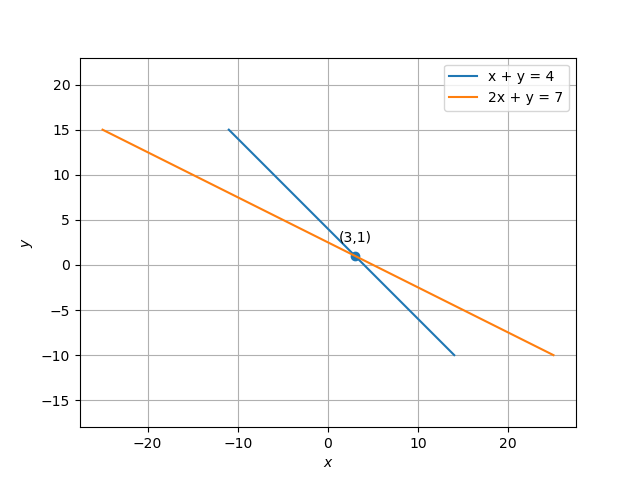
\includegraphics[width=\columnwidth]{chapters/11/10/1/11/figs/line.png}
		\caption{}
		\label{fig:11/10/1/11}
  	\end{figure}
	\iffalse
\vspace{5mm}
%-----------------------------solution---------------------------
\raggedright \textbf{SOLUTION}:\vspace{2mm}\\

%---------given----------------%
\raggedright \textbf{Given}:\vspace{2mm}\\
Slope of one line is double of the slope of the other line. \\\vspace{1mm}
\fi
\\
\solution 
The direction vector of a line is expressed as
\begin{align}
\vec{m}=\myvec{1\\m}
\end{align}
where  $m$ is defined to be the slope of the line. If the angle between the lines be $\theta$,
\begin{align}
\tan \theta = \frac{1}{3}
\implies \cos \theta=\frac{3}{\sqrt{10}}
\end{align}
\iffalse
%--------------steps----------------------%
\textbf{Input Parameters:}
\vspace{2mm}


\begin{tabular}{|c|c|c|}
	\hline
	\textbf{Symbol}&\textbf{Value}&\textbf{Description}\\
	\hline
	$\vec{m_1}$ &\myvec{1\\m}& Direction vector\\
	\hline
    $\vec{m_2}$ &\myvec{1\\2m}&Direction vector\\
	\hline
    $\tan\theta$ &1/3& Angle\\
	\hline
\end{tabular}
\\
\vspace{10cm}
\fi
The angle between two vectors is then expressed as
\iffalse
\begin{align}
\cos \theta = \frac{^\top \textbf{B}}{\norm{\textbf{A}}\norm{\textbf{B}}}
\end{align} 
%Substituting the \vec{m_1} and \vec{m_2} in the above equation
\\
\fi
\begin{align}
	\frac{3}{\sqrt{10}} &= \frac{\vec{m}_1^\top \vec{m}_2}{\norm{\vec{m}_1}\norm{\vec{m}_2}}
	\\
	&= \frac{\myvec{1 &  m}\myvec{1 \\ 2m}}{\norm{\myvec{1\\m}}\norm{\myvec{1\\2m}}}
\\
	&= \frac{2m^2 +1}{\sqrt{m^2 + 1}\sqrt{4m^2 + 1}}
	\\
	\implies \frac{9}{10}&=\frac{4m^4 + 4m^2 +1}{4m^4 + 5m^2 +1}
\\
	\text{or, } 4m^4 - 5m^2 +1 = 0
\end{align}
\iffalse
Let $m^2$ = x and substituting it in above equation we get a quadratic equation.
\begin{align}
	4x^2 -5x +1 = 0
\end{align}
From the formula of fining roots of a quadratic equation
\begin{align}
	\frac{-b\pm \sqrt{b^2 - 4ac}}{2a}
	\\
	\\
	\frac{5\pm \sqrt{\left (-5\right )^2 - 16}}{8}
	\\
	x= 1 (or) x = 1/4
\end{align}
\\
The slope of the first line is
\\
\fi
yielding
\begin{align}
m=\pm \frac{1}{2}, 
\pm 1
\end{align}
\iffalse
$\therefore $ Slope of second line is
\begin{center}
$ 2m=\pm 1$\\
    (or)\\
    $2m=\pm 2$
\end{center}
\begin{center}
 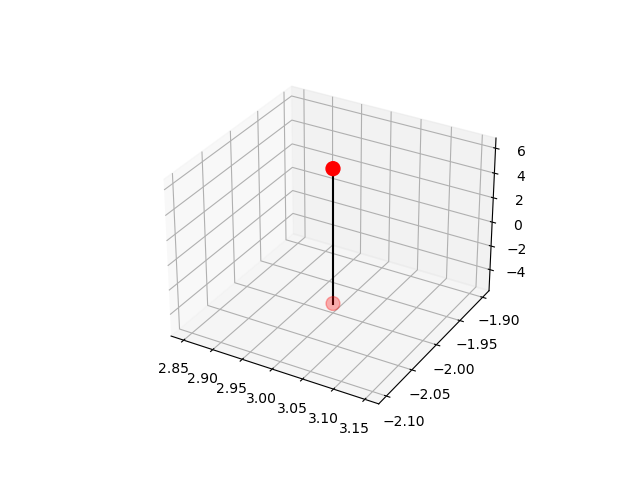
\includegraphics[width=0.5\textwidth]{line.png}  
 \end{center}\vspace{1mm}
\raggedright  Download the code \\
Github link:{Assignment-4}.
\end{multicols}
\end{document}
\fi

\item    Find angle between the lines,$\sqrt{3}x+y=1$ and $x+\sqrt{3}y$=1.
\label{chapters/11/10/3/9}
\iffalse
\def\mytitle{LINE ASSIGNMENT}
\def\myauthor{G.Kumar}
\def\contact{kumargandhamaneni20016@gmail.com}
\def\mymodule{Future Wireless Communication (FWC)}
\documentclass[10pt, a4paper]{article}
\usepackage[a4paper,outer=1.5cm,inner=1.5cm,top=1.75cm,bottom=1.5cm]{geometry}
\twocolumn
\usepackage{graphicx}
\graphicspath{{./images/}}
\usepackage[colorlinks,linkcolor={black},citecolor={blue!80!black},urlcolor={blue!80!black}]{hyperref}
\usepackage[parfill]{parskip}
\usepackage{lmodern}
\usepackage{tikz}
\usepackage{physics}
\usepackage{tabularx}
\usetikzlibrary{calc}
\usepackage{amsmath}
\usepackage{amssymb}
\renewcommand*\familydefault{\sfdefault}
\usepackage{watermark}
\usepackage{lipsum}
\usepackage{xcolor}
\usepackage{listings}
\usepackage{float}
\usepackage{titlesec}
\providecommand{\mtx}[1]{\mathbf{#1}}
\titlespacing{\subsection}{1pt}{\parskip}{3pt}
\titlespacing{\subsubsection}{0pt}{\parskip}{-\parskip}
\titlespacing{\paragraph}{0pt}{\parskip}{\parskip}
\newcommand{\figuremacro}[5]{
    \begin{figure}[#1]
        \centering
        \includegraphics[width=#5\columnwidth]{#2}
        \caption[#3]{\textbf{#3}#4}
        \label{fig:#2}
    \end{figure}
}
\newcommand{\myvec}[1]{\ensuremath{\begin{pmatrix}#1\end{pmatrix}}}
\let\vec\mathbf
\lstset{
frame=single, 
breaklines=true,
columns=fullflexible
}
\thiswatermark{\centering \put(0,-105.0){
\includegraphics[scale=0.35]{iith}} }
\title{\mytitle}
\author{\myauthor\hspace{1em}\\\contact\\IITH\hspace{0.5em}-\hspace{0.5em}\mymodule}
\date{}
\begin{document}
	\maketitle
\section*{Problem}
\fi
   \\
   \solution 
   \iffalse
   \section*{Solution}
   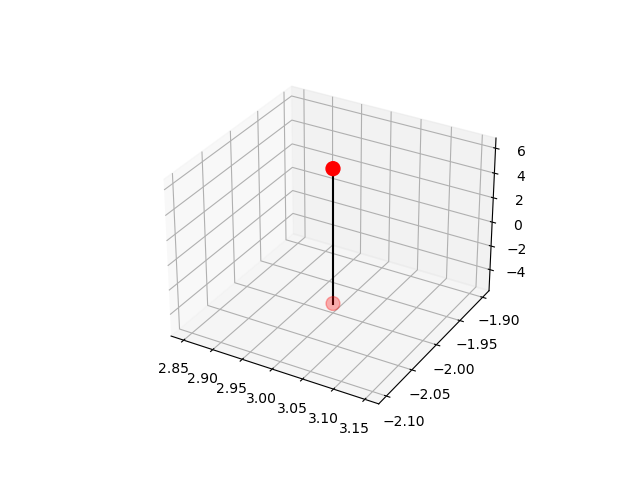
\includegraphics[scale=0.55]{line.png}
   The input parameters for this construction are :
   \begin{center}
\begin{tabular}{|c|c|c|}
	\hline
	\textbf{Symbol}&\textbf{Value}&\textbf{Description}\\
	\hline
	P&$\
	\begin{pmatrix}
		0.57736 \\
		0 \\
	\end{pmatrix}$%
	&Point P\\ 
	\hline
	X&$\
	\begin{pmatrix}
		0.36603 \\
		0.36603 \\
	\end{pmatrix}$%
	&Point X\\
	\hline
	Q&$\
	\begin{pmatrix}
		1 \\
		0 \\
	\end{pmatrix}$%
	&Point Q\\
	
	\hline
\end{tabular}
\end{center}
   \subsection*{Step 1}
   Given two equations are, \\
   \begin{equation}
   \sqrt{3}x+y=1 
   \end{equation}
   \begin{equation}
   x+\sqrt{3}y=1 
   \end{equation}
   Equation(1) in vector form is given as,
   \fi
From    the given equations, the normal vectors can be expressed as
\iffalse
   \begin{align}
   \myvec{\sqrt{3}&1}\vec{x}=1
   \end{align}
   From this, Normal vector to the line is given as,
   \fi
   \begin{align}
	   \vec{n}_1=\myvec{\sqrt{3}\\1},
	   \vec{n}_2=\myvec{1\\\sqrt{3}}
   \end{align}
   \iffalse
   So, the direction vector of the line is given as,
\begin{eqnarray*}
   \vec{m2}=\myvec{-\sqrt{3}\\1}
\end{eqnarray*}     

\subsection*{Step 2}
Now, Angle between any two lines,using their direction vectors, is given by, \\
\fi
The angle between the lines can then be expressed as
\begin{align}
	cos\theta&=\frac{\vec{n}_1^T\vec{n}_2}{\norm{\vec{n}_1}\norm{\vec{n}_2}}
	\\
	&=\frac{\sqrt{3}}{2} 
	\\
	\text{or, }
\theta=30\degree
\end{align}
\iffalse
\begin{eqnarray}
 cos\angle{x}=\frac{(\vec{m1})^T(\vec{m2})}{\norm{\vec{m1}}\norm{\vec{m2}}}\
\end{eqnarray}
\begin{eqnarray}
 cos\angle{x}=\frac{\myvec{-1\\\sqrt{3}}^T\myvec{-\sqrt{3}\\1}}{\norm{\myvec{-1\\\sqrt{3}}}\norm{\myvec{-\sqrt{3}\\1}}}
\end{eqnarray}
By solving the above equation, we get, \\
\begin{equation}
cos\angle{x}=\frac{\sqrt{3}}{2} \\
\end{equation}
This Implies,
\begin{equation*}
\angle{x}=30^\circ
\end{equation*}
Therefore, the angle between given two lines is $30^\circ$. \\
\bibliographystyle{ieeetr}
\end{document}
\fi

\end{enumerate}
